El álgebra booleana, al igual que todos los sistemas matemáticos deductivos, se define con
un conjunto de elementos, un conjunto de operadores y varios axiomas o postulados no
demostrados. Un conjunto de elementos es cualquier colección de objetos con alguna propiedad
en común.

\subsection{Elementos del álgebra booleana}
\begin{itemize}
    \item \textbf{0 y 1:} Son los dos elementos básicos del álgebra booleana. Se les llama
    elementos binarios o bits. El 0 representa el estado de apagado o falso, mientras que el 1
    representa el estado de encendido o verdadero.
    \item \textbf{Variables:} Son símbolos que representan cantidades desconocidas o no
    especificadas. En el álgebra booleana, las variables pueden tomar uno de los dos valores
    posibles, 0 o 1.
\end{itemize}

\subsection{Teoremas y postulados del álgebra booleana}
Los teoremas y postulados que se presentan son las relaciones más básicas del álgebra
booleana. Los teoremas, al igual que los postulados, se presentan por pares; cada relación es
el dual de su pareja. Los postulados son axiomas básicos de la estructura algebraica y no requieren demostración. Los teoremas deben demostrarse a partir de los postulados.

\begin{figure}[h]
\centering
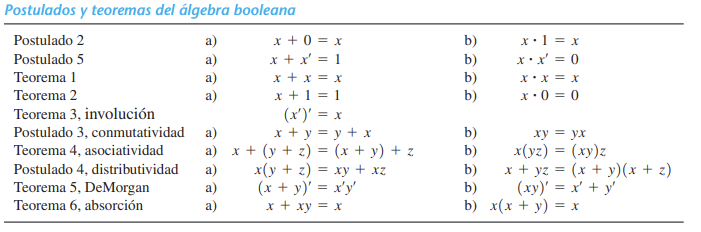
\includegraphics[scale=1]{img/teopol.png}
\end{figure}

\subsection{Funciones booleanas}
El álgebra booleana es un álgebra que se ocupa de variables binarias y operaciones lógicas. Una función booleana descrita por una expresión algebraica consta de variables binarias, las constantes 0 y 1, y los símbolos lógicos de operación. Para un valor dado de las variables binarias, la función puede ser igual a 1 o bien a 0.

\begin{mdframed}[backgroundcolor=gray!10,linewidth=0]
    Una función booleana expresa la relación lógica entre variables binarias. Se evalúa determinando el valor binario de la expresión para todos los posibles valores de las variables. Podemos representar una función booleana en una tabla de verdad. Una tabla de verdad es una lista de combinaciones de unos y ceros asignados a las variables binarias y una columna que muestra el valor de la función para cada combinación binaria. El número de filas de la tabla es $2^n$, donde $n$ es el número de variables de la función. Las combinaciones binarias para la tabla de verdad se obtienen de los números binarios, contando de $0$ hasta $2^n -1$. 
\end{mdframed}

\newpage
Por ejemplo, supongamos que se tiene la función: $F_1 = x + y'z$:

La tabla de la verdad es la siguiente:
\begin{figure}[h]
\centering
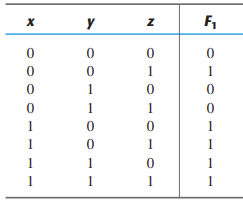
\includegraphics[scale=1]{img/tbvdd.png}
\end{figure}

Y la implementación de la función en un circuito lógico sería:
\begin{figure}[h]
\centering
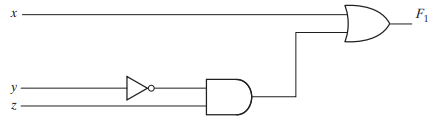
\includegraphics[scale=0.9]{img/imple.png}
\end{figure}

\subsection{Compuertas Lógicas digitales}
Puesto que las funciones booleanas se expresan en términos de operaciones \texttt{AND}, \texttt{OR} y \texttt{NOT}, es más fácil implementar una función booleana con estos tipos de compuertas. La posibilidad de construir compuertas para las otras operaciones lógicas tiene interés práctico.

Cada compuerta tiene una o dos variables binarias de entrada designadas con $x$ y $y$, y una variable binaria de salida designada con \texttt{F}. 

\begin{figure}[h]
\centering
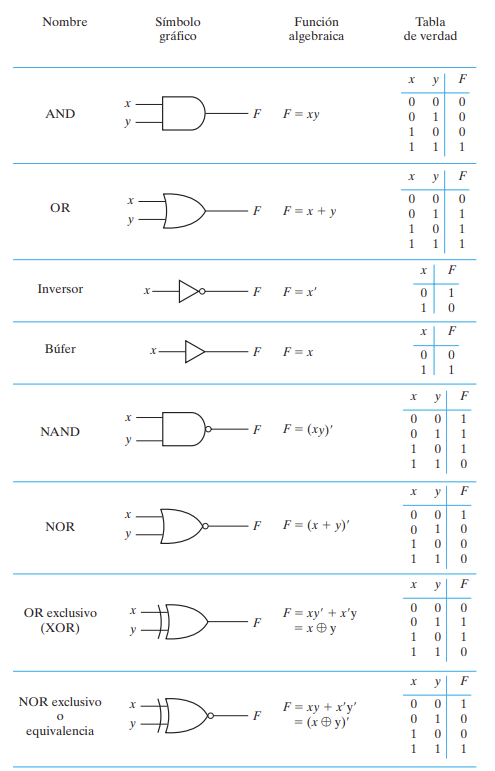
\includegraphics[scale=0.75]{img/comp.png}
\end{figure}

